\documentclass{article}
\usepackage{tikz}
\usepackage{lipsum} % For dummy text (can be removed if not needed)

\begin{document}

\section*{Introduction to Intercepts of a graph and how to identify them}

\vspace{1em} % Add a little vertical space after the section title

\begin{minipage}[c]{0.45\textwidth} % Minipage for the text
    1. A balloon is rising from a ravine, it starts 13 ft below ground

    \vspace{1em} % Add some vertical space between items

    2. A ball is falling from the sky, then bounces off the ground then falls back down and stops

    \vspace{1em} % Add some vertical space between items

    3. You are standing on a 7 ft tall platform and you spin a yo-yo downwards.
\end{minipage}
\hfill % Horizontal fill to push minipages apart
\begin{minipage}[c]{0.45\textwidth} % Minipage for the TikZ graph
    \centering % Center the TikZ picture within its minipage
    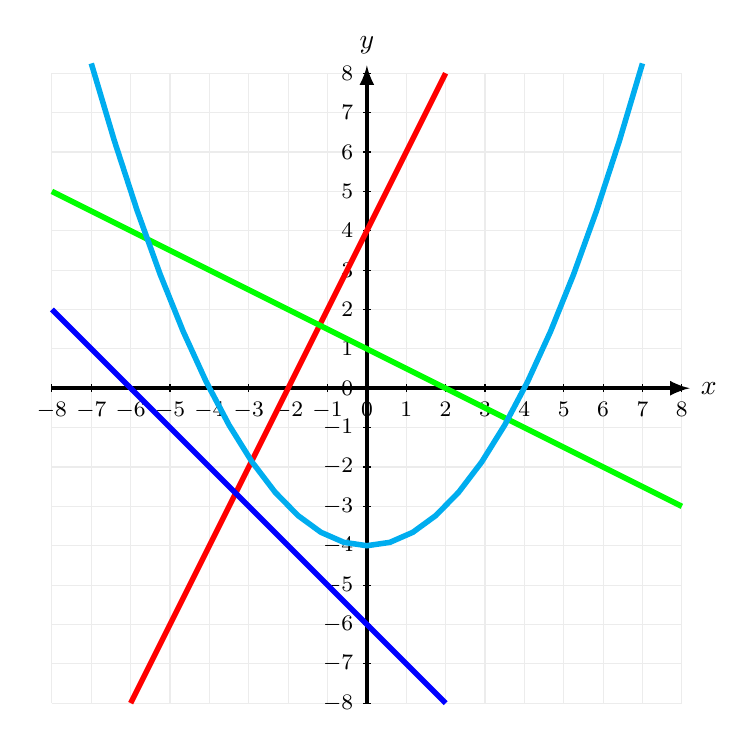
\begin{tikzpicture}[scale=0.50]
        \draw[gray!15,step=1cm] (-8,-8) grid (8,8);
        \draw[line width=0.5mm, -latex] (-8,0) -- (8.2,0) node[right] {$x$};
        \foreach \x in {-8,...,8} \draw (\x,.1)--(\x,-.1) node[below] {\footnotesize $\x$};
        \draw[line width=0.5mm,  -latex] (0,-8) -- (0,8.2) node[above] {$y$};
        \foreach \y in {-8,...,8} \draw (.1,\y)--(-.1,\y) node[left] {\footnotesize $\y$};
        \draw[red,line width=2pt] plot[domain= -6:2] (\x,{2*\x+4});
        \draw[blue,line width=2pt] plot[domain= -8:2] (\x,{-1*\x-6});
        \draw[green,line width=2pt] plot[domain= -8:8] (\x,{-0.5*\x+1});
        \draw[cyan,line width=2pt] plot[domain= -7:7] (\x,{0.25*\x*\x-4});
    \end{tikzpicture}
\end{minipage}

\end{document}